\documentclass{report}

\usepackage{fancyhdr} % Cabeceras de página
\usepackage{lastpage} % Módulo para añadir una referencia a la última página
\usepackage{titling} % No tengo claro para qué es esto
\usepackage[left=3cm,right=2.5cm,top=3cm,bottom=2cm]{geometry} % Márgenes
\usepackage[T1]{fontenc}
\usepackage[utf8x]{inputenc}
\usepackage{xspace}
\usepackage{graphicx}
\usepackage{tikz}
\usepackage{wrapfig}
\usepackage{hyperref}

\hypersetup{
  hyperindex,
    colorlinks,
    allcolors=blue!60!black
}


\setcounter{secnumdepth}{3}


\title{Fault Manager Lite - Technical report}
\date{\today}
\author{{\Large Triforce} \\ \vspace{5pt} \textit{Iván Márquez Pardo, Víctor de Juan Sanz, Guillermo Julián Moreno} \\ v1.0 - Draft}

\fancyhf{}
\fancypagestyle{plain}{%
	\lhead{\small \itshape \thetitle\, -\, \thedate\, -\, SEPRO}
	\rhead{\vspace{-20pt} 
\includegraphics[width =40 pt]{../Logo.jpg}}
	\cfoot{\thepage\ of \pageref{LastPage}}
	\rfoot{}
}

\begin{document}
\maketitle
\tableofcontents
\newpage
\pagestyle{plain}
\begin{abstract}
\end{abstract}

\chapter{Introduction}

The Autonomous University of Madrid (UAM) has reported the numerous problems it has on detecting faults that arise on its campus and its facilities, whose reparation usually takes excessive time and is poorly organized. A late detection of faults in the facilities delays its reparation, stopping its users to continue using them as normal and complicating the maintenance staff labour. Regarding the wishes of the campus users and realizing the maintenance problems it has, the UAM has organised a contest to choose the best project proposal that solves them.
This is where our organization, Triforce, enters the scene: we have analysed the problem exhaustively and designed a web application, Fault Manager Lite (FML), that meets all the requirements expected, solves the problems and also includes new extra features that makes it even more useful.

\paragraph{Purpose} The purpose of this Software Requirements Specification (SRS) document is to provide a detailed description of the functionalities of the FML system. This document will cover each of the system's intended features, as well as offer a preliminary glimpse of the software application's User Interface (UI).

\section{Structure}

In this chapter, we introduce you to the purpose of this document, some definitions and the methodology used during the development of this proposal.

An exhaustive definition of this project can be found on chapter \ref{chapProjectDefinition}, where we state the goals of the system, its functionalities and the proposed modules.

All the requirements are detailed in the chapter \ref{chapRequirements}, where functional and non-functional requirements are specified, explained and justified.

Chapter \ref{chapDesign} defines the visual design of the application, stating the motivation for our choices and the user experience that will be delivered with this project.

Finally, we conclude with chapter \ref{chapConclusions}, where we will sum up all the points exposed in this report and will present compelling reasons for why our proposal should be the chosen one.

As annexes, in appendix \ref{chapBrainstorming} we write down the transcription of our initial brainstorming, the seed of this proposal. We evaluate the current technology that could be used to solve the UAM's problems in appendix \ref{chapCurrentTechnology}, and in appendix \ref{chapMeetings} we reproduce the announcements and minutes of our meetings. We also include the interview with the UAM's maintenance administrator in appendix \ref{chapInterview}


\section{Definitions and abbreviations}

\begin{itemize}
\item \textbf{SRS: } Software Requirements Specification.

\item \textbf{FML: } Fault Manager Lite. This is the System's name.

\item \textbf{UAM: } \textit{Universidad Autónoma de Madrid}, Madrid's Autonomous University, the client for whom this project will be developed.

\item \textbf{GUI: } Graphical User Interface.

\item \textbf{GPS: } Global Positioning System.

\item \textbf{SQL: } Structured Query Language, often used as synonymous of relational database systems.

\item \textbf{Devops: } Team responsible for the deployment and maintenance of the software.

\end{itemize}


\section{Methodology}

The methodological procedure followed for preparing the SRS of the software system FML we have developed includes the following techniques:
\begin{enumerate}
\item Deep analysis of the information given by the UAM: the potential maintenance problem it has, the causes that led to this problem and various aspects we must consider before proceeding to the next step (web application that must work on PCs, tablets and smartphones; target users; basic purpose).
\item Application of the technique of brainstorming to generate ideas for the application. Brainstorming was then applied to these general ideas in order to give shape to them. The results of the brainstorm carried out are shown in the Annex \ref{chapBrainstorming}. This step resulted on the detection of 5 subsystems.
\item Research on the Internet about other similar systems, analyzing the functionality of these systems and describing them in a structured way by specifying their advantages and disadvantages, and extracting good ideas to incorporate to our own project, increasing its market value. These ideas also helped putting the final touches to our ideas from the brainstorm.
\item Interview with one member of the UAM's technical staff. In this interview we clarified the obscure ideas we still had, and modified some of our previous ideas to adapt them to the answers given. The answers to the interview were well-considered; as the technical staff will be the main user of our application, their point of view is important to us. The interview it is included in annex \ref{chapInterview}.
\item Departing from the ideas obtained, defined the requirements (functional and non-functional) of the application and design attractive mock-ups that fulfill them. These mock-ups are only a demo and may change in the final version of the application.
\end{enumerate}

\chapter{Project Definition}
\label{chapProjectDefinition}

FML is based on the jolly cooperation between the users of the facilities of the UAM campus and the maintenance staff in charge of them.

As the users will be the ones that will detect the sooner faults on the facilities the campus offers them, they are also the most suitable to report the problems they are having, in order to getting them fixed as soon as possible. With the FML web application, it will only take less than a minute to fill the form and send it to the maintenance staff.

Using the reports of faults detected in the campus, the maintenance personnel will stop losing its precious time revising the installations looking for faults and will be able to focus on the repairs. Apart from this benefit, the maintenance staff will also have a better way to coordinate efforts, as the FML will provide an automatic assignment system to assign repairs to each of the members avoiding overloading any of them and taking into account their distance to the problem, saving time on displacements.

In summary, the users will be able to easily report faults on facilities they are using in order to have them fixed in the less time possible, while the maintenance personnel will multiply its current performance as the majority of their resources will stop being wasted on revisions, but on repairs. We state that the FML web application is the answer to the UAM problems, as we will show you with this SRS.


\section{Goals and functionalities}

Our main goal is the development of an extremely functional, bug-free web application, that runs either on PCs, tablets or smartphones and facilitates the labor of the maintenance staff of the UAM.

Based on the jolly cooperation between the members of the UAM community (students, teaching and research staff and administration and services personnel) and the maintenance personnel of the facilities and installations of the UAM campus, this application has been designed to solved the potential maintenance problems that the UAM has declared to have.

The problems we aim to alleviate with this application include the following:


\begin{itemize}
\item Difficulty of detecting faults on facilities of the campus.
\item Late detection of the problems, which implies repairs are not done on time.
\item Excessive resources and time wasted on revisions looking for potential faults.
\item Bad coordination between members of the technical staff.
\item Frequent overloading of some repairmen because of bad coordination.
\item Inability of a repairman to instantly inform that a fault has just been solved.
\item Difficulty of the users to report faults to the maintenance services.
The report system lacks of mobile functionality.
\item Lack of real-time visualization of pending and finished repairs.
\item Lack of real-time visualization of assigned tasks.
\item No faults history.
\item No statistics of faults.
\end{itemize}

\section{Subsystems or Modules}

The FML system has been designed to resolve these problems making use of a user-friendly interface, avoiding unnecessary or distracting buttons or effects. This system has been divided in several modules listed below, each of those offering one specific functionality and, in conjunction, solving the problems mentioned above:
\begin{itemize}
\item Task Manager.
\item Report System.
\item Notifications and Messaging System.
\item Users and Profile Managers.
\item Faults History.
\end{itemize}

There are several applications 'on the market' which are similar to our proposed app in some way or another and they could represent real and competitive alternatives to ours. However, none of these web applications can offer all the features FML offers (furthermore, we plan on adding some features which are not currently available in any of these applications), so our system is indeed the best solution proposed to solve the problems the UAM maintenance staff has to deal with. After our research of the Internet, a comparison of these competitors applications is gathered in Annex \ref{chapCurrentTechnology}.

% -*- root: ../Technical_report.tex -*-
\chapter{Catalog of Requirements}
\label{secRequirements}

Before we start defining FML's requirements we need to define two things, the \textbf{roles} inside FML and the \textbf{Operating environment} in which FML will work.


\label{chapRequirements}
\section{Roles}

\paragraph{Reporter role} \label{ReporterRole} This is the role applied to anyone who want to report some fault. It will be taken into account the person's status inside UAM community (student, PhD, teacher, maintenance technician, etc). Every user in FML's system will be able to report faults.

\paragraph{Maintenance Personnel} \label{MaintenancePersonnel}

These are the roles applied to people in charge of maintenance. Inside maintenance personnel we need to distinguish 2 subcategories:

\begin{itemize}
\item Boss: The people in charge of each department.
\item Maintenance technician: The maintenance personnel responsible to fix the faults.
\end{itemize}

As there are 8 departments, there will be 8 categories, listed below:

\begin{itemize}
\item Heating.
\item Plumbing.
\item Air conditioning.
\item Cleaning.
\item Information Technologies.
\item Elevators.
\item Electricity.
\item Trash Collection.
\item Gardeners.
\end{itemize}

Each maintenance person should be tagged in, at least, 1 department. It is also compatible being boss and technician.

\paragraph{Exceptions} The \textbf{cleaning department} only needs a person in charge of the whole department and it is his responsibility to assign faults to their employees and to mark faults as solved.

This department is also special because there is a different department in each faculty, so the must be at least 1 person in charge of each faculty cleaning department. As we mentioned before, maintenance personnel can also report faults.

\paragraph{Administrator Role} Is the person (or group of people) in charge of UAM's maintenance system in general. Every administrator will have permissions to change everything within the application, as they are in charge of everything related with maintenance.

\section{Operating environment}

The main component of Fault Manager Lite is the application, HTML based, that will run in PCs, tablets and smartphones. To improve usability and integration with operating systems, a native application wrapping the HTML interface will be developed so the users won't need to run the browser in order to access the application.

The system will require a backend exposing a RESTful API to which the HTML clients will connect. Separation of concerns is important in order to improve maintainability and ability to respond quickly to user feedback.

The server will require an installation of Python 3, and a working connection to a SQL server. Our application will be independent of the specific implementation of the server (database maintenance will be responsibility of the devops\footnote{I.e., the University's IT team.} team).

Specific implementation details are out of the scope of this proposal, but we will develop the application with scalability in mind: the interface, API and database applications will be independent and loosely coupled in order for the devops team to deploy each one to as many machines as needed. Cloud deployments are an option, but is not required (actually, we recommend using the university datacenter in order to comply with spanish privacy laws).

\section{Requirements}

\subsection{Functional requirements}

\subsubsection{Task Manager subsystem}

\paragraph{Faults definition} Each fault will have 3 possible states: \textit{Pending to assign, assigned, solved}.

If a fault is impossible to be fixed, it will correspond to the administrator to take care personally of it.


\paragraph{Categorizing faults} There should be categories to tag each fault depending on the priority (low, medium or high) and the department who needs to take care of it. The system will assign automatically a priority to each fault, although the administrators will be able to change it at any point in time.

\paragraph{Fault's assignments} FML will assign to maintenance personnel faults to be fixed (depending on the fault's category and maintenance person load of work and capability to solve the fault)

This will be set automatically and the system's administrators will be able to reassign the faults as they pleased.

The person in charge of a department will also be able to reassign faults that have been assigned to his department or to someone inside his department to his employees.

As we mentioned before, the cleaning departments are special, because all cleaning faults in a building will be assign to the person in charge of that building's cleaning.


\paragraph{Task managing} Everyone from the maintenance personnel will have read access to the faults data base through a Graphical User Interface (GUI).

They will just have write access to faults they have been assigned to. \footnote{Write access is needed so the maintenance person change fault's state to \textit{solved} or to \textit{in progress}}

Admin will have write access to all faults in the system, and the person in charge of a department will have write access to all faults assigned to someone inside his department.

\paragraph{When a fault is fixed} The maintenance person assigned (or the manager of that department) will mark as solved the fault. At that time, the reporter will get notify and thanked.


\subsubsection{Report subsystem}

\paragraph{Reporting a fault} Our system will allow:

\begin{itemize}
\item Reporting a fault with the following information: \textit{Location, date, priority\footnote{The actual priority will be set automatically taking into account this priority, the one reported by the user, and other parameters, such as the user's history of reports.}, category, photograph (optional) and description}.

\item See and check reported faults and see its state.

\item Answer questions the maintenance personnel will ask about the reported fault.
\end{itemize}


\paragraph{Duplicated faults} This is a big problem to be solved. What we propose to solve it has 2 aspects.
\begin{itemize}
\item FML will be able to mark as \textit{possible duplicated}, so all possible duplicates will be assign to the same maintenance people, so he can verify if they are duplicated or not.

\item On the other side, to prevent duplicated faults reports, FML will show a message showing possible duplicated faults to the reporter. If the reporter marks the fault he is reporting as duplicated, he will earn some points too and will be added into the list of people to be notified when the task is solved.
\end{itemize}


\subsubsection{Communication subsystem - Notifications and messaging}

\paragraph{Communication} Maintenance person assigned to fix a fault should be able to ask the fault's reporter for more information.


\subsubsection{Users and Profile manager system}

\paragraph{Log in} Everyone must be able to login using UAM credentials. We will use the service provide by UAM to authenticate an user.

If the user is logging in on a smartphone, the system shouldn't ask for the password more than once (except for some specific operations defined in the role-depending requirements, user role category (\ref{Specifics_Secure_Requirements_for_user}))

\paragraph{Updating profile} What if a student become a teacher and then his email needs to be changed? To fix this, every user must be able to update his profile's information.


\subsubsection{Faults History}

\paragraph{Seeing history} As we think transparency is really important, every reporter will be able to see all history of faults. In non-functional requirements we define how this should be done.

\paragraph{Statistics} In the profile page each user should be able to see the faults he has reported and it's state.

Plus, he should be able to see his conversations with maintenance personnel.


\subsection{Non-Functional}

\subsubsection{General Requirements}

This requirements are defined for all roles inside FML (Administrator, maintenance personnel and user)

\paragraph{Profile} Everyone should have a profile with some private information such as name or email.

\paragraph{Lightweight application} FML will be lightweight enough to run in 4 years old Chrome, Firefox, IE's versions.

\paragraph{Read Access to task} Every FML's user will be able to see all reported faults (we think transparency is really important). This will be shown on a map of the UAM. Each fault will appear as an arrow pointing to fault's location and color-tagged depending on its state (solved, pending, assigned).

\subsubsection{Role-depending requirements}

\paragraph{Reporter} FML should provide users the following abilities:
\begin{itemize}
\item The specifics requirements where re-authentication is needed are: \textit{Answering questions asked by maintenance personnel}   \label{Specifics_Secure_Requirements_for_user} and \textit{updating profile information}.
\item The interface to report a fault should be easy enough to let the user report the fault without losing much time.
\item The amount of points earned should be visible inside profiles page. It will be also shown the conversion in ECTS credits so the user knows how much he have earned.

\end{itemize}



\chapter{Design and Mock-ups}
\label{chapDesign}

\section{Motivation}

This application's purpose is to solve a problem, not to create new. Thus, the design should not interfere with the technicians or the users work. Instead, it must reduce friction to almost zero, so it has to be easy to use and easy to learn. Adoption by the student corp of the application is critical to this project, so the design should accommodate to this requirement.

We want the application to be full-featured, so all the users of the app should be able to use all the features from whichever device they're working in: tablet, smartphone or PC. We don't want anybody to stop reporting a fault because they don't have their laptop with them, for example.

This leads to a natural decision regarding the technologies used to develop the interface: we will use web technologies and responsive design to maximize code reuse. In this way, we will be able to deliver a high quality user experience and homogeneous among devices with minimal code and improved maintainability.

In turn, this will allow us to reduce costs and will make the development more agile, as we will be able to deliver quickly changes to the application responding to feedback from users.


\begin{figure}[hbtp]
\centering
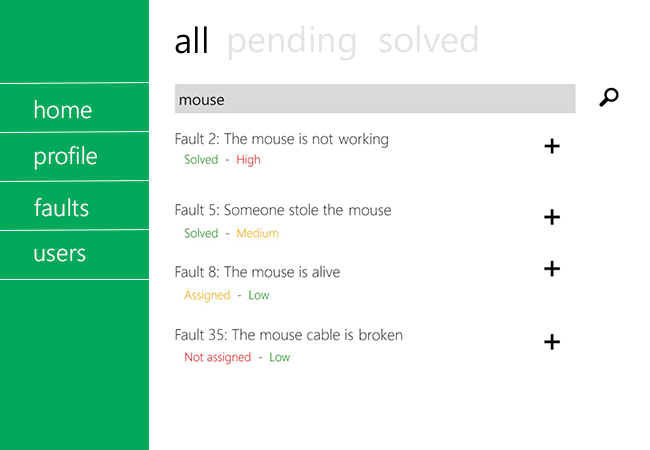
\includegraphics[width=0.8\textwidth]{img/WideScreens.png}
\caption{Sample responsive design in wide screens (laptops, tablets in landscape position, PCs) with the menu showing up and large interface elements .}
\label{imgWideScreens}
\end{figure}

In this report, we will include, for brevity, the mockups for a mobile application, as we consider it will be the most used interface for the system. Given that we will be using responsive design, the looks will be the same for every device, except for widened interface elements and a navigation menu that shows up if there's enough space (see figure \ref{imgWideScreens} compared with the corresponding mobile view on figure  \ref{imgFaultLog}).

\section{Design}

\begin{figure}[hbtp]
\centering
\begin{minipage}{0.3\textwidth}
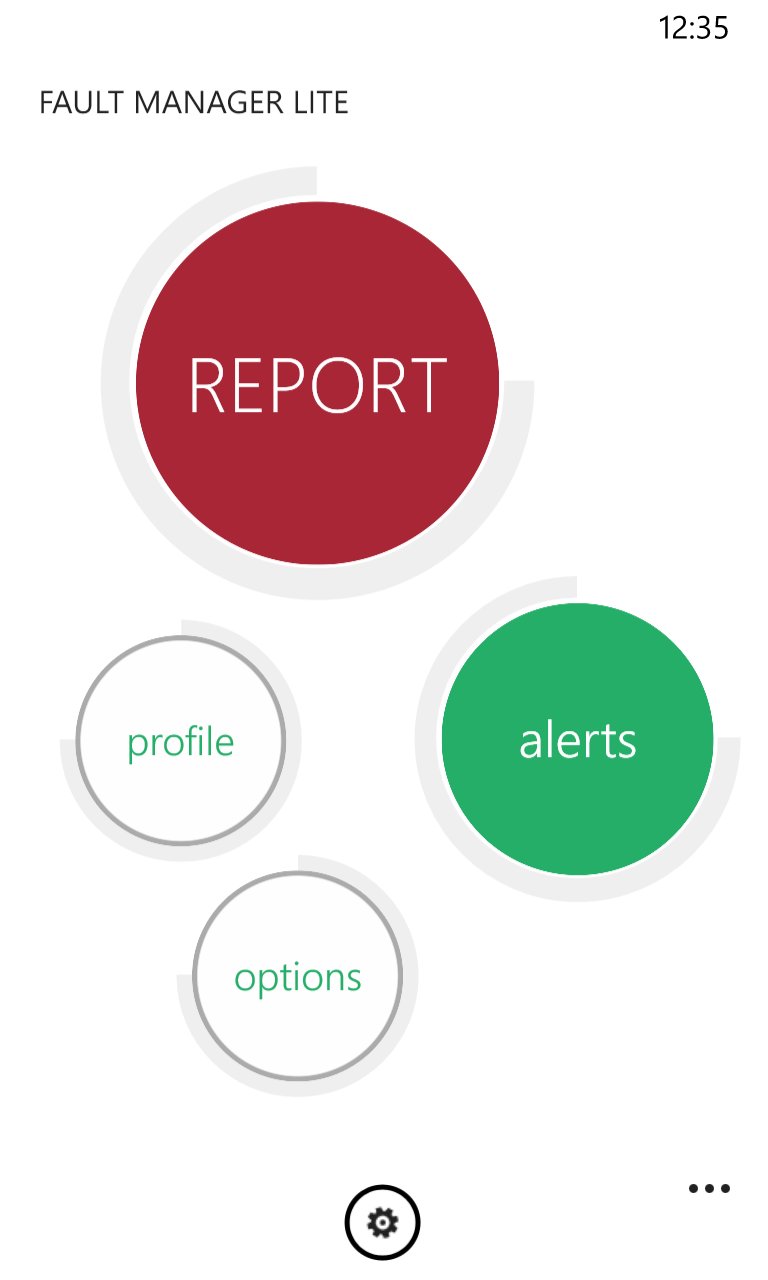
\includegraphics[width=\textwidth]{img/MainPage.png}
\end{minipage}
\hspace{0.1\textwidth}
\begin{minipage}{0.3\textwidth}
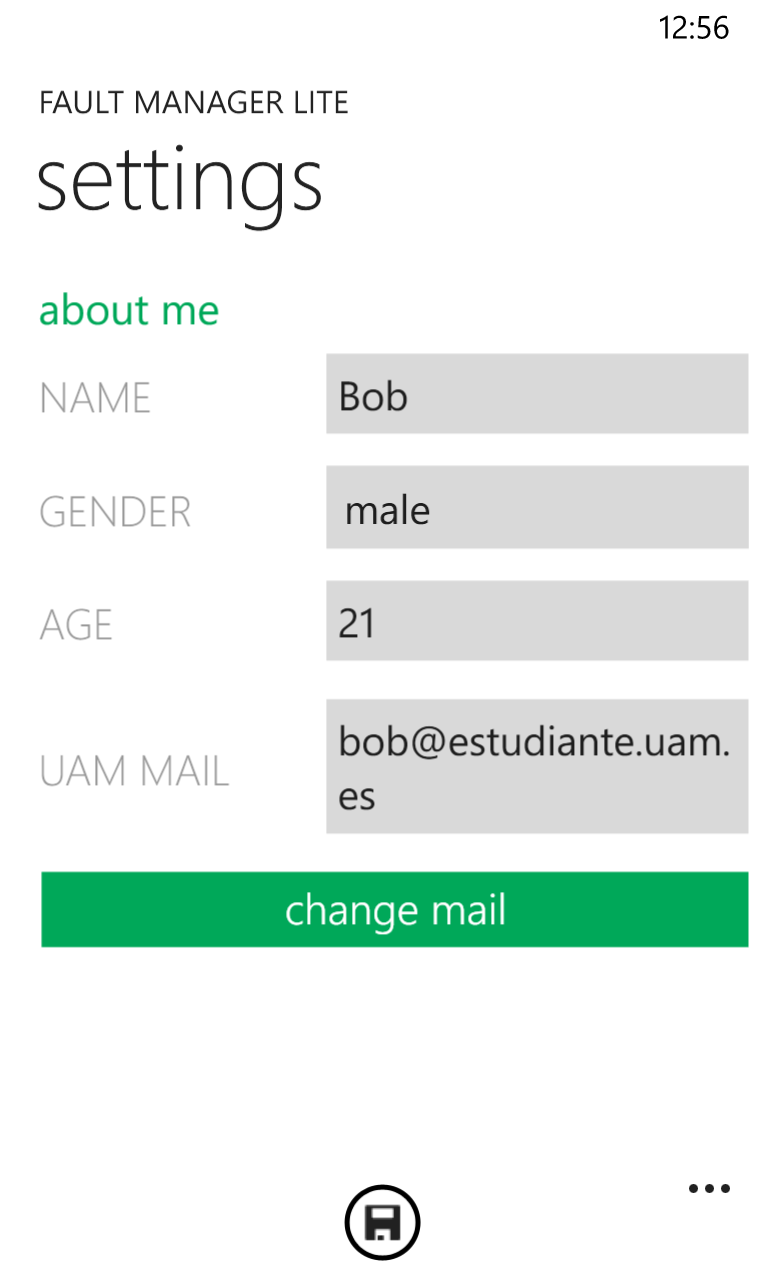
\includegraphics[width=\textwidth]{img/Settings.png}
\end{minipage}
\caption{Main page and settings page for Fault Manager Lite}
\label{imgMainPage}
\end{figure}

We show some mock-ups of the application, specifically designed to show the flow in certain use cases.

\subsection{Reporting a fault}

From the main screen (figure \ref{imgMainPage}), when the user presses the button ``Report'', he will be able to choose a category for the fault, then will fill the details and then get a page acknowledging the report and showing the estimated response time (figure \ref{imgReportFlow}). They may see a message popup (\ref{imgDuplicateReport}) if a possible duplicated report is detected.

\begin{figure}[hbtp]
\centering
\begin{minipage}{0.3\textwidth}
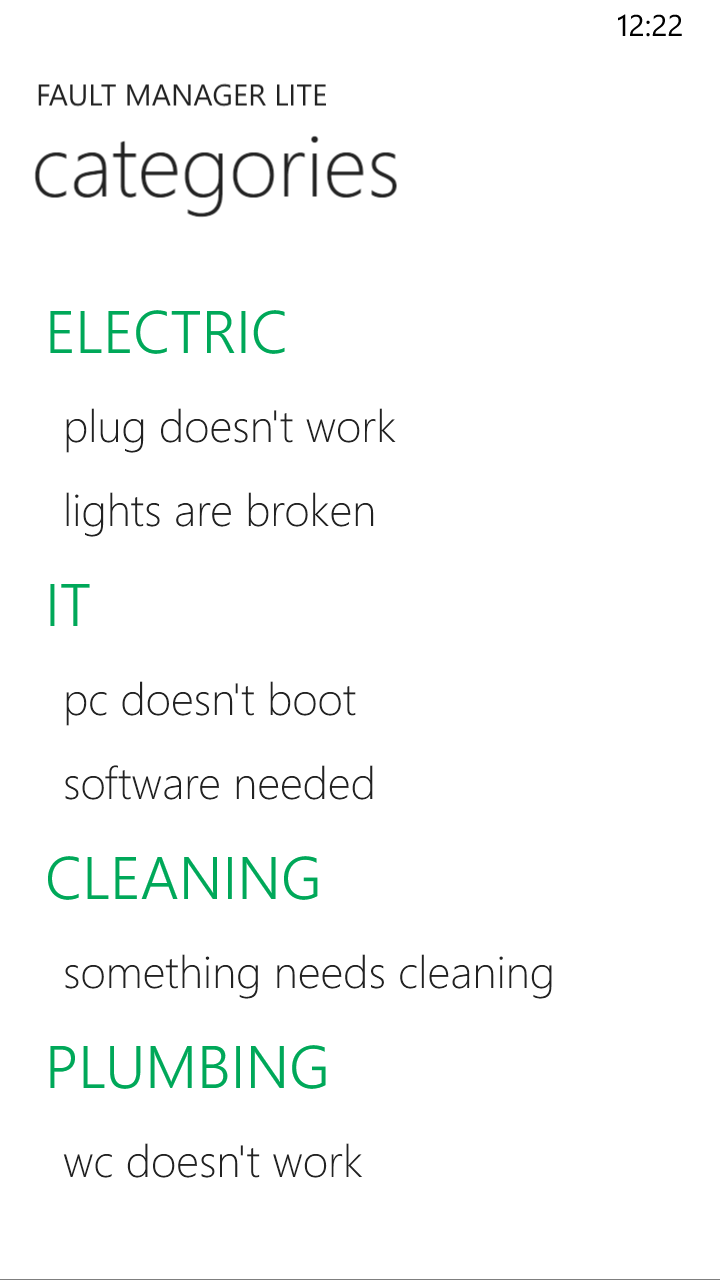
\includegraphics[width=\textwidth]{img/Categories.png}
\end{minipage}
\hspace{0.02\textwidth}
\begin{minipage}{0.3\textwidth}
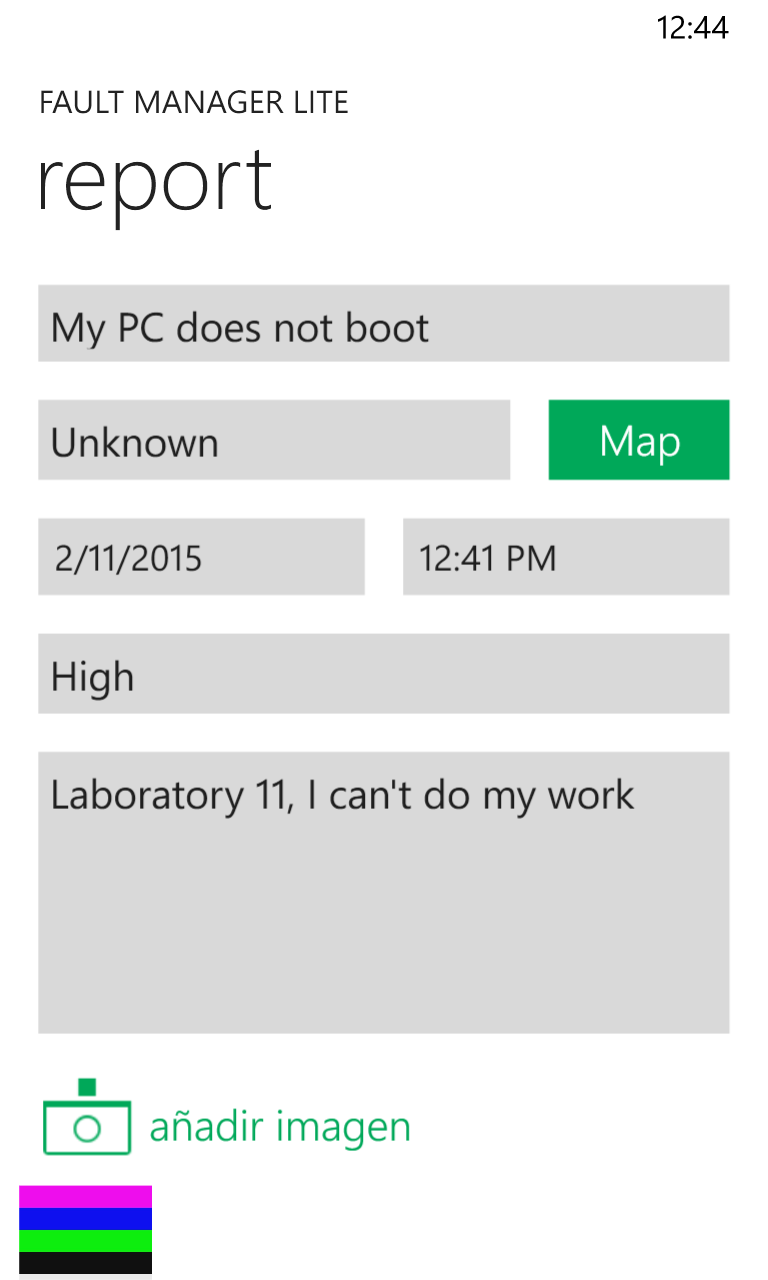
\includegraphics[width=\textwidth]{img/ReportPage.png}
\end{minipage}
\hspace{0.02\textwidth}
\begin{minipage}{0.3\textwidth}
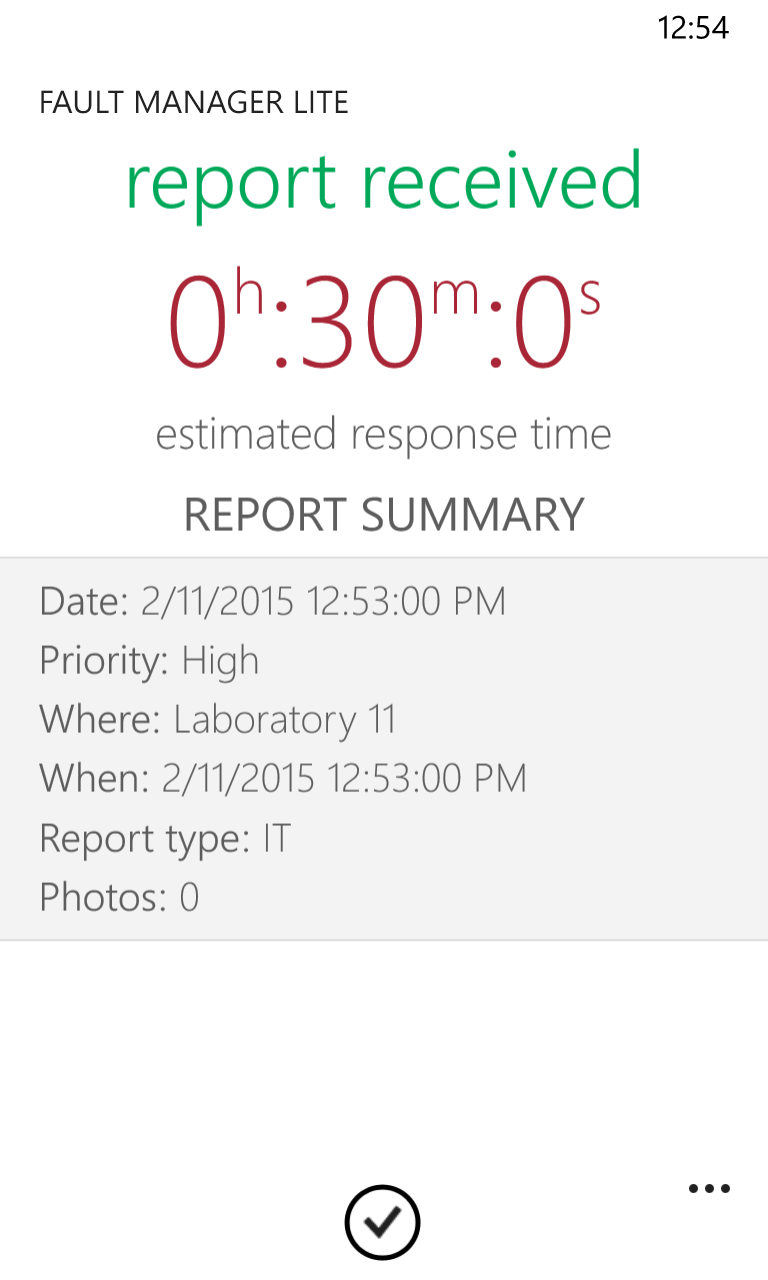
\includegraphics[width=\textwidth]{img/ReportReceived.png}
\end{minipage}
\caption{Basic flow for reporting a fault.}
\label{imgReportFlow}.
\end{figure}

\begin{figure}[hbtp]
\centering
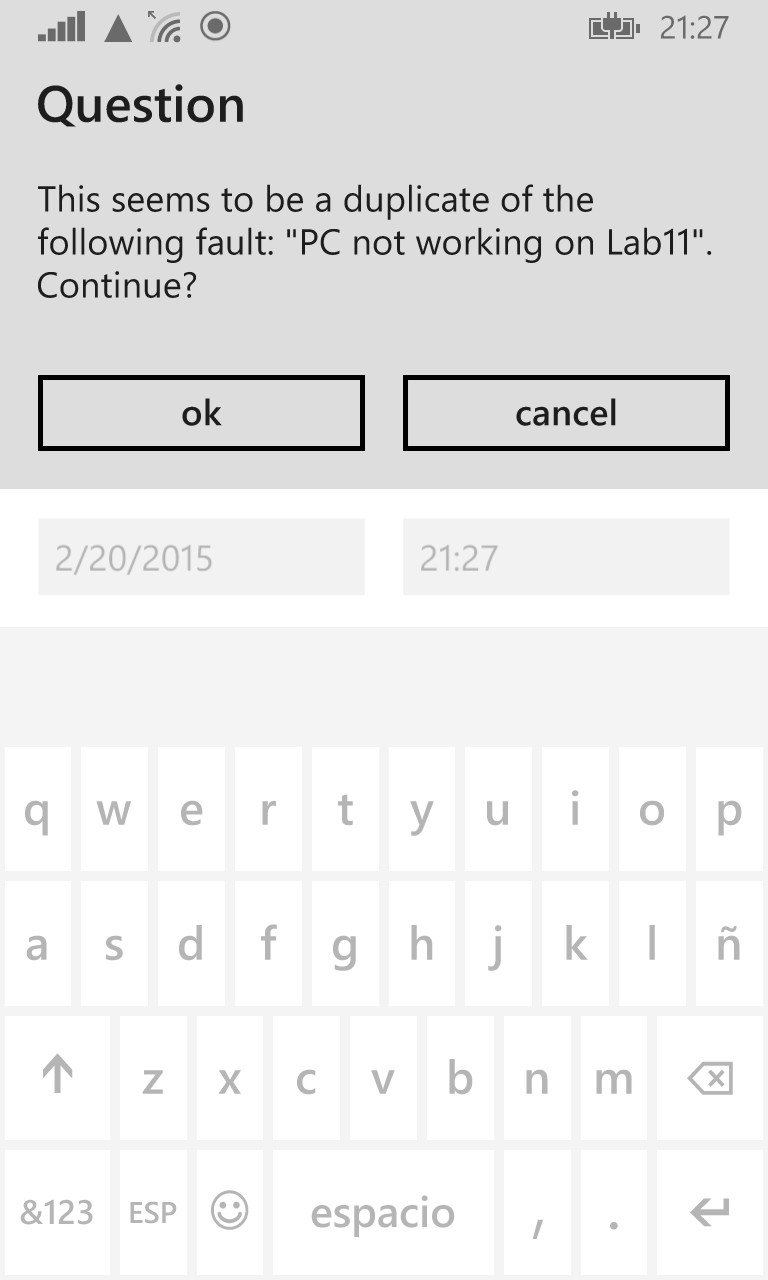
\includegraphics[width=0.3\textwidth]{img/DuplicateMessage.jpg}
\caption{When a possible duplicate is found, the user is asked if he or she wants to continue with the report.}
\label{imgDuplicateReport}
\end{figure}

For the location, we will show the user a map and also a list with all the possible options (figure \ref{imgLocation}). The user will be able to select specific places (for example, a certain lab or classroom) or more generic (e.g., third floor or the whole building). If localization APIs are available on the device (either location by AGPS or WiFi), the application will use them to show the user the best location option.


\begin{figure}[hbtp]
\centering
\begin{minipage}{0.3\textwidth}
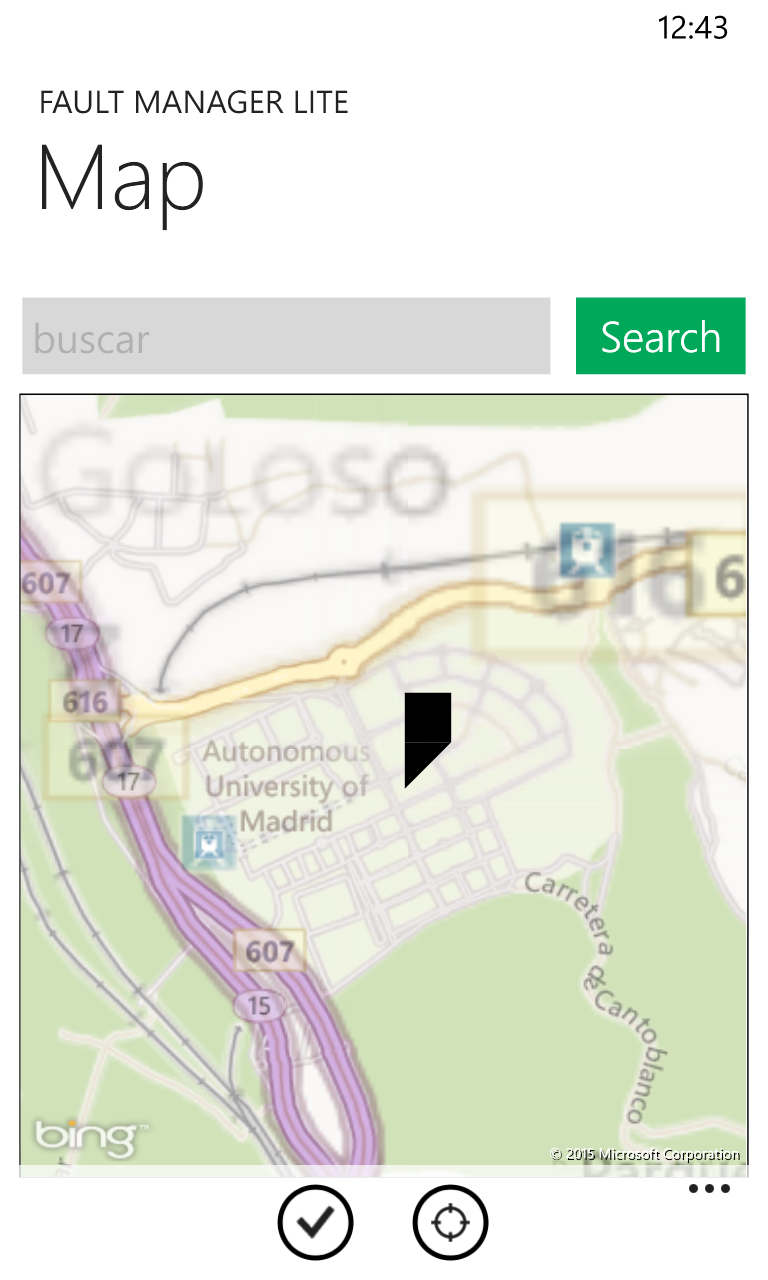
\includegraphics[width=\textwidth]{img/Map.png}
\end{minipage}
\hspace{0.02\textwidth}
\begin{minipage}{0.3\textwidth}
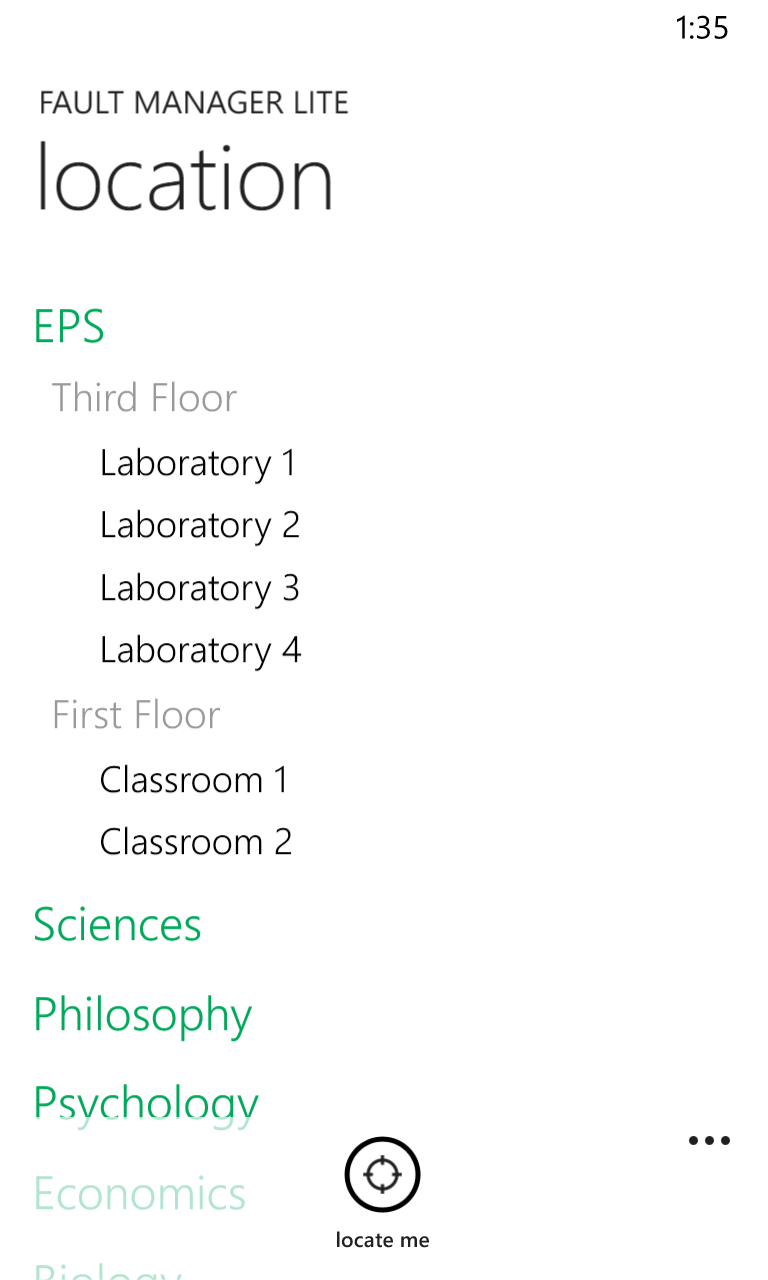
\includegraphics[width=\textwidth]{img/Location.png}
\end{minipage}
\caption{Location screens for the application}
\label{imgLocation}
\end{figure}

\subsection{Fault tracking}

\begin{figure}[hbtp]
\centering
\begin{minipage}{0.3\textwidth}
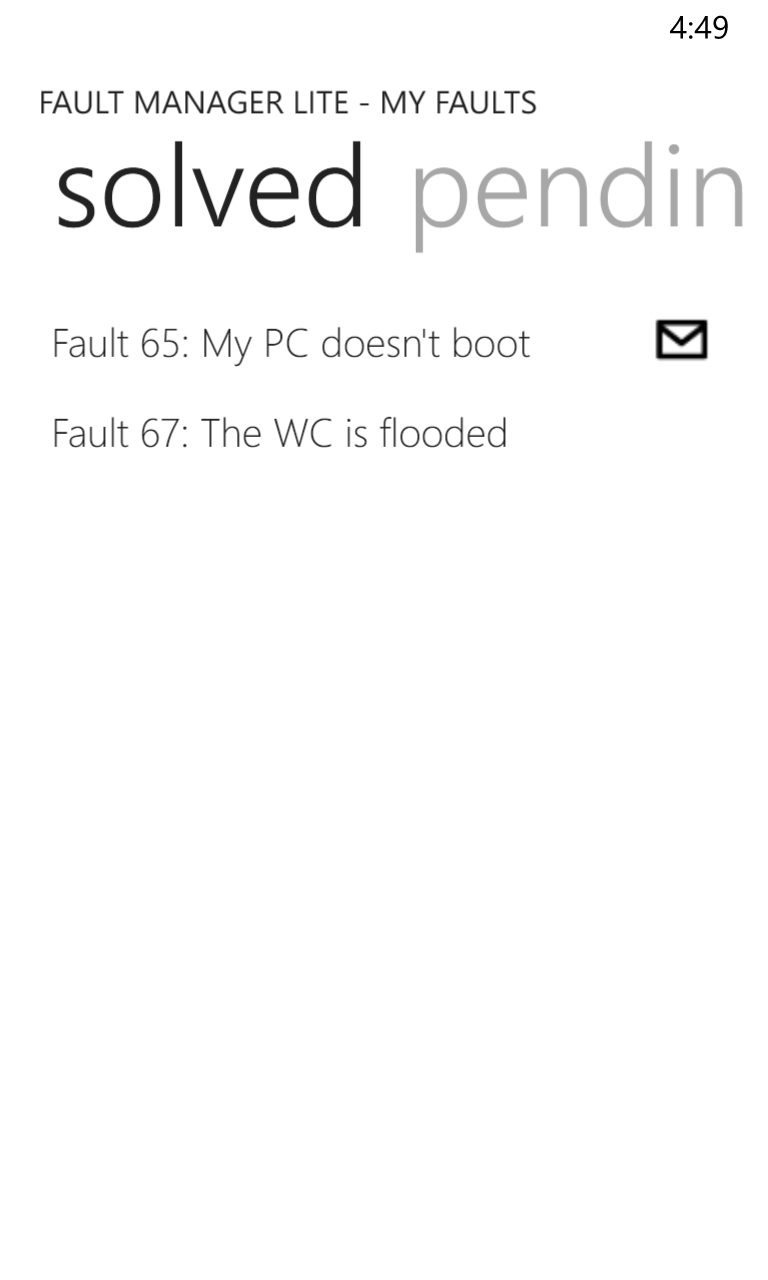
\includegraphics[width=\textwidth]{img/FaultLog.png}
\end{minipage}
\hspace{0.02\textwidth}
\begin{minipage}{0.3\textwidth}
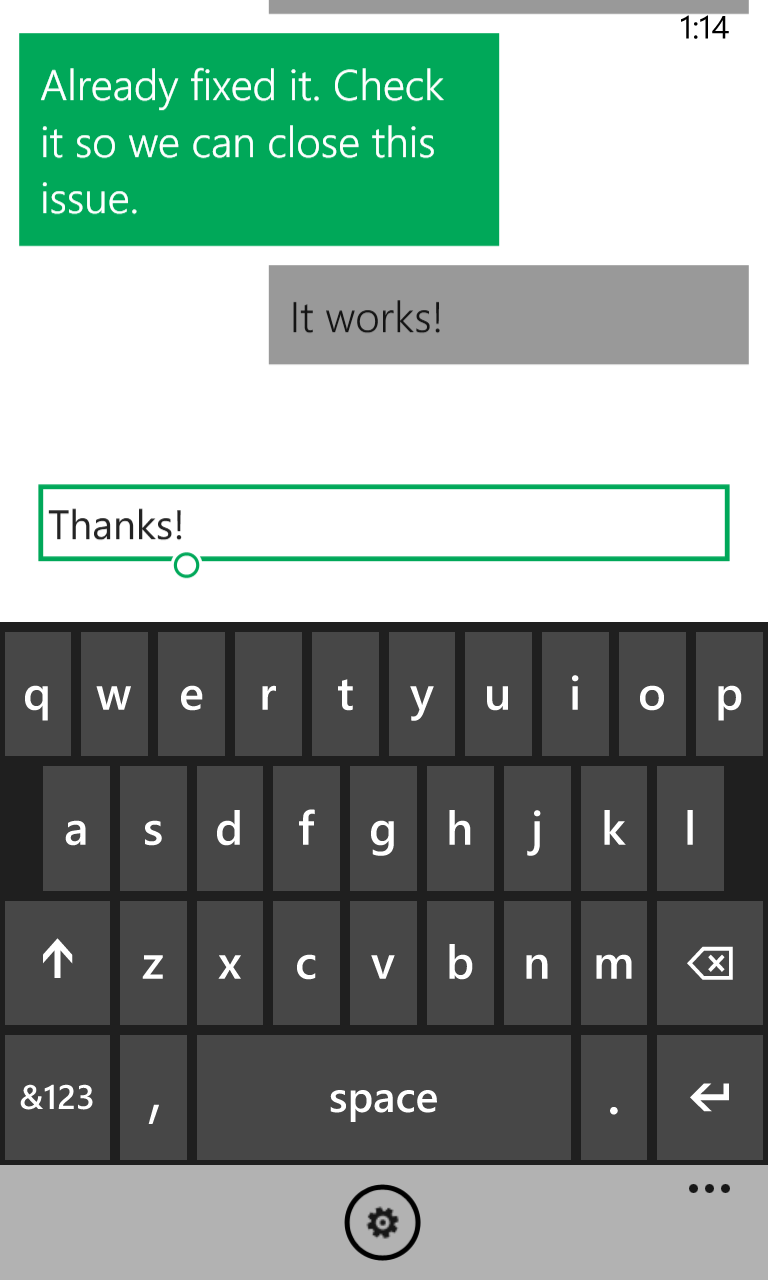
\includegraphics[width=\textwidth]{img/Messaging.png}
\end{minipage}
\caption{Fault log and messaging screen for the application.}
\label{imgTracking}
\end{figure}

The user will be able to see the faults he's been subscribed too, either because he reported them or because he marked them as duplicated. The figure \ref{imgTracking} shows how can he see all his faults and the chat screen that will show up if the technicians need to clarify details of the report.


\begin{figure}[hbtp]
\centering
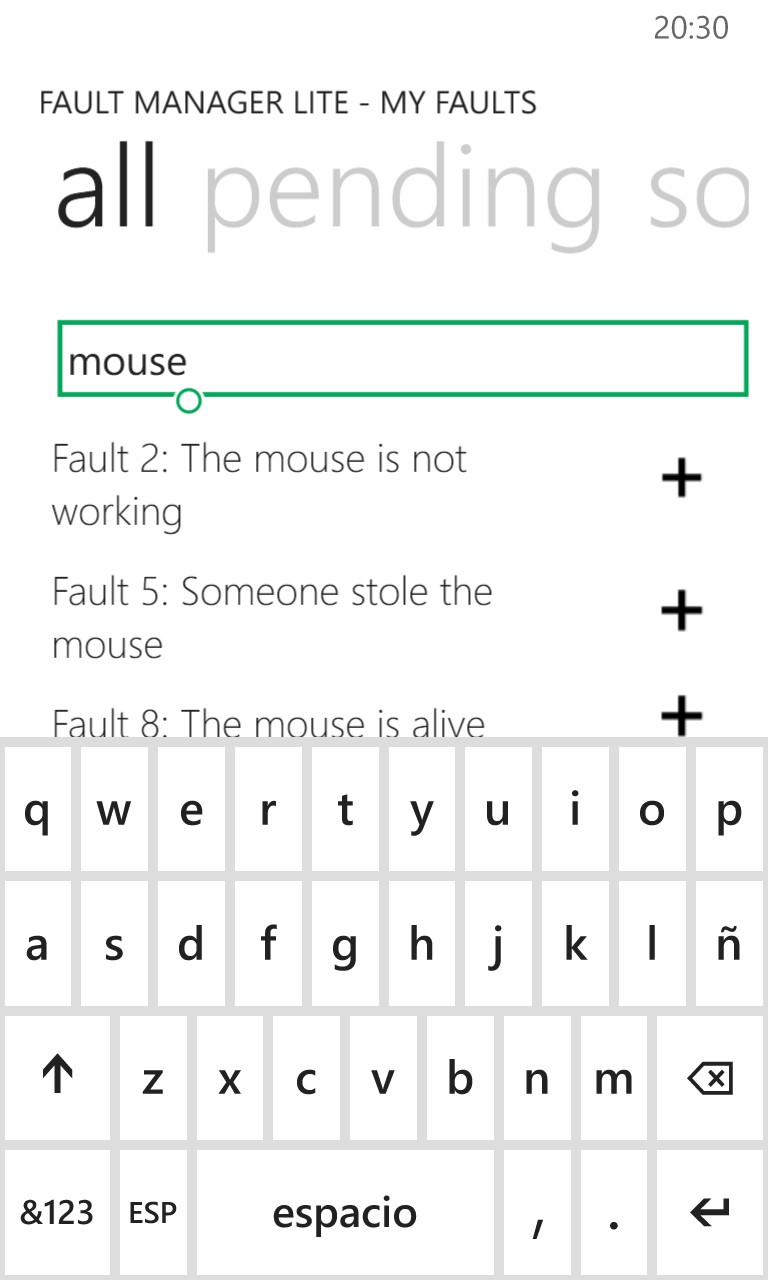
\includegraphics[width=0.3\textwidth]{img/AllFaults.jpg}
\caption{The users can see all the faults.}
\label{imgAllFaults}
\end{figure}

As specified on the requirements, the users will be able to see all the faults in the system (figure \ref{imgAllFaults}). To improve usability, we will include a search option so the users can find teh reports they're interested in.

\subsection{Interface for technicians}

\begin{figure}[hbtp]
\centering
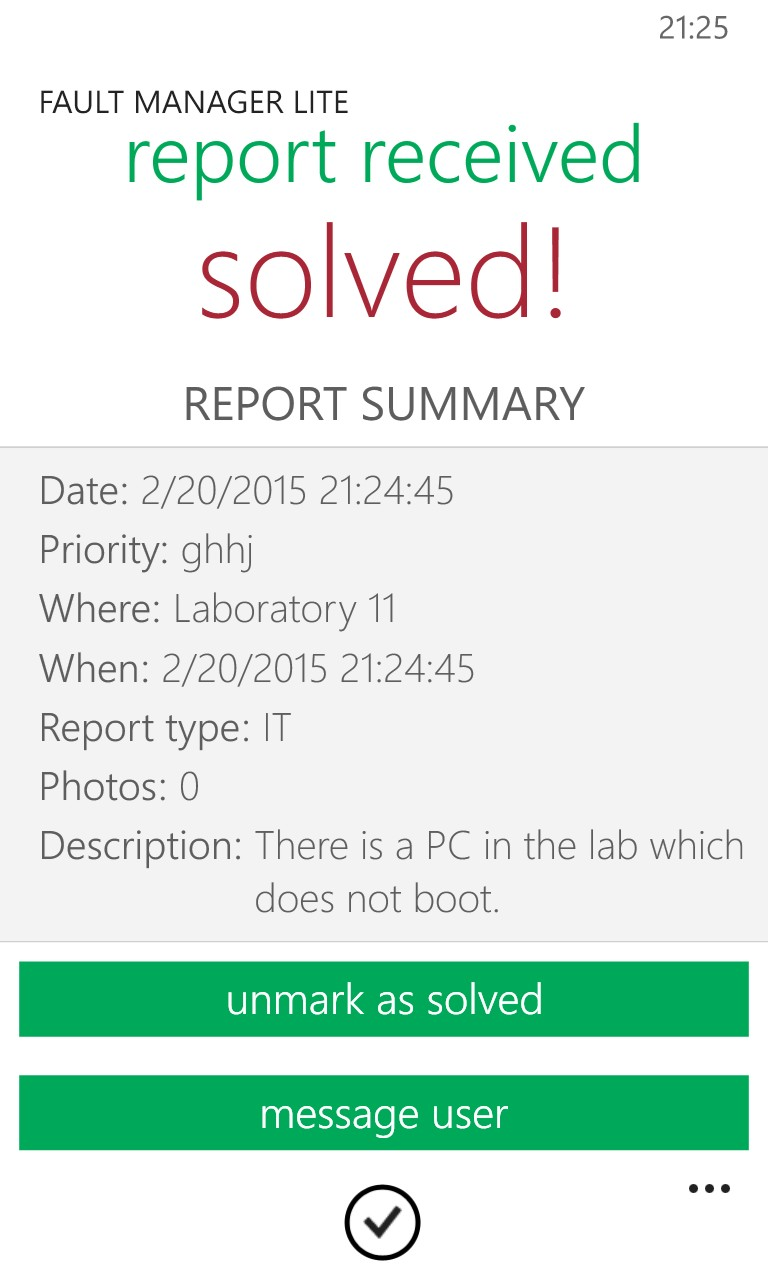
\includegraphics[width=0.3\textwidth]{img/SolvedFault.jpg}
\caption{The technicians will have controls to mark a fault as solved or communicate with the users.}
\label{imgSolvedFault}
\end{figure}

To reduce costs and improve mantainability, most of the code and interface will be shared between user roles. This means that the common screens (main screen, settings, fault lists and report information) will be the same for technicians, with maybe some additional elements (see figure \ref{imgSolvedFault}).

The technicians will be able to see their assigned tasks in a slightly modified interface of the one normal users see (figure \ref{imgFaultLog}), so they will be able to check the priority and state of the fault. The contextual menu of each task will allow the user to mark the fault as duplicate or assign it to someone (if the technician hasn't got managing responsibilities, he will only be able to assign the to him/herself).

\begin{figure}[hbtp]
\centering
\begin{minipage}{0.3\textwidth}
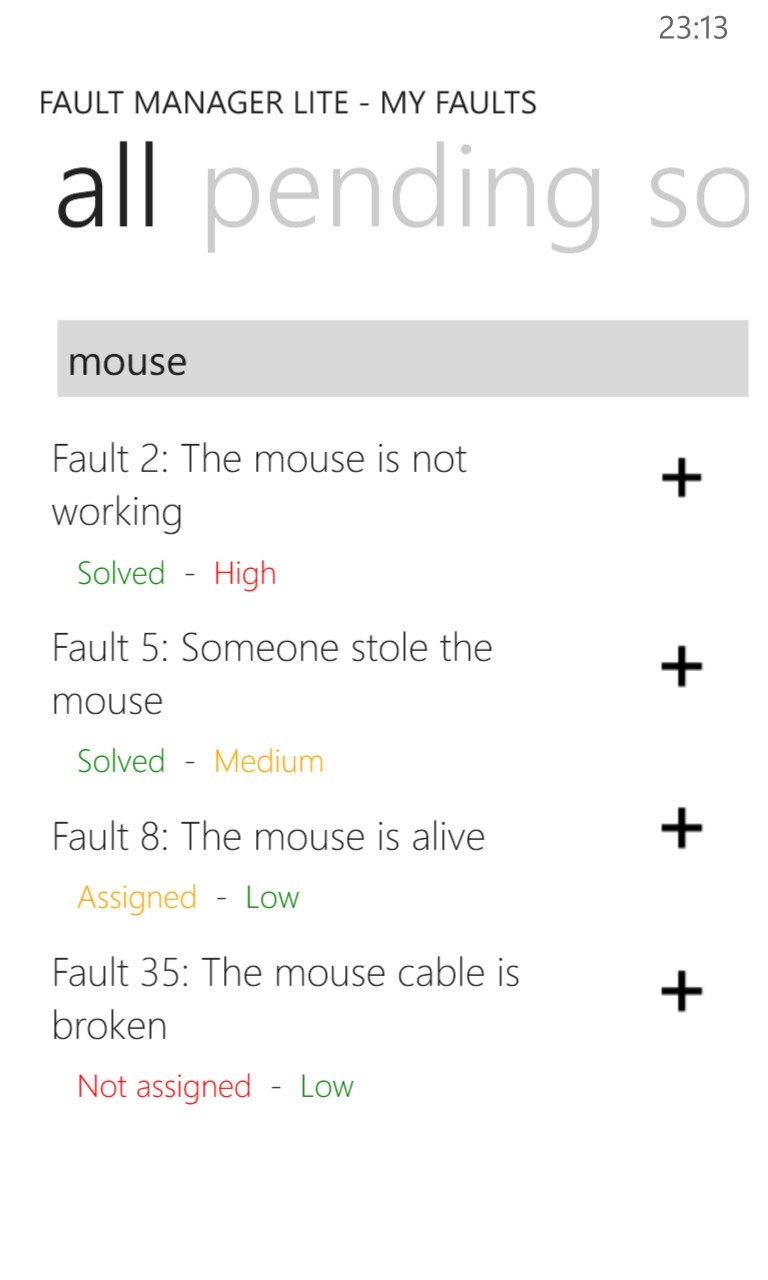
\includegraphics[width=\textwidth]{img/TechFaultLog.jpg}
\end{minipage}
\hspace{0.02\textwidth}
\begin{minipage}{0.3\textwidth}
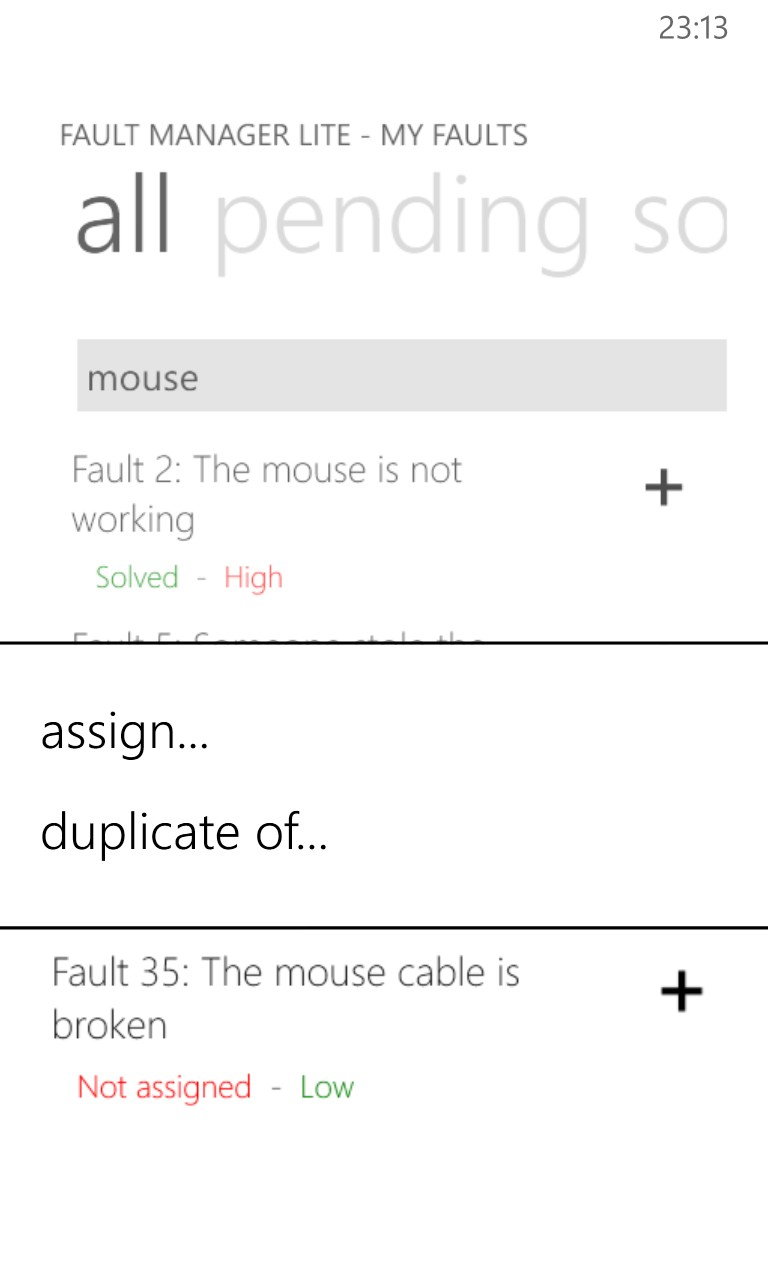
\includegraphics[width=\textwidth]{img/TechAssign.jpg}
\end{minipage}
\caption{The technicians will see additional information in the faults page.}
\label{imgFaultLog}
\end{figure}

\subsection{Interface for admins}

\begin{figure}[hbtp]
\centering
\begin{minipage}{0.3\textwidth}
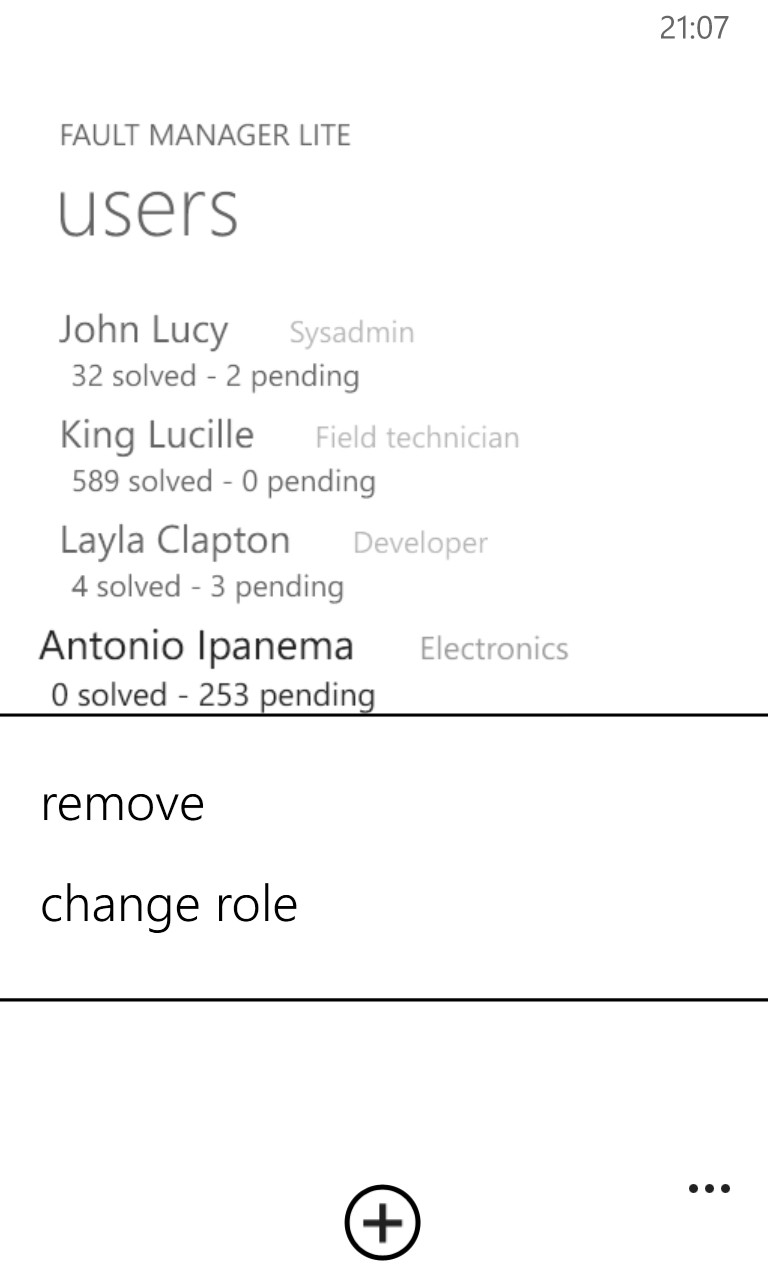
\includegraphics[width=\textwidth]{img/AssignRemoveUser.jpg}
\end{minipage}
\hspace{0.02\textwidth}
\begin{minipage}{0.3\textwidth}
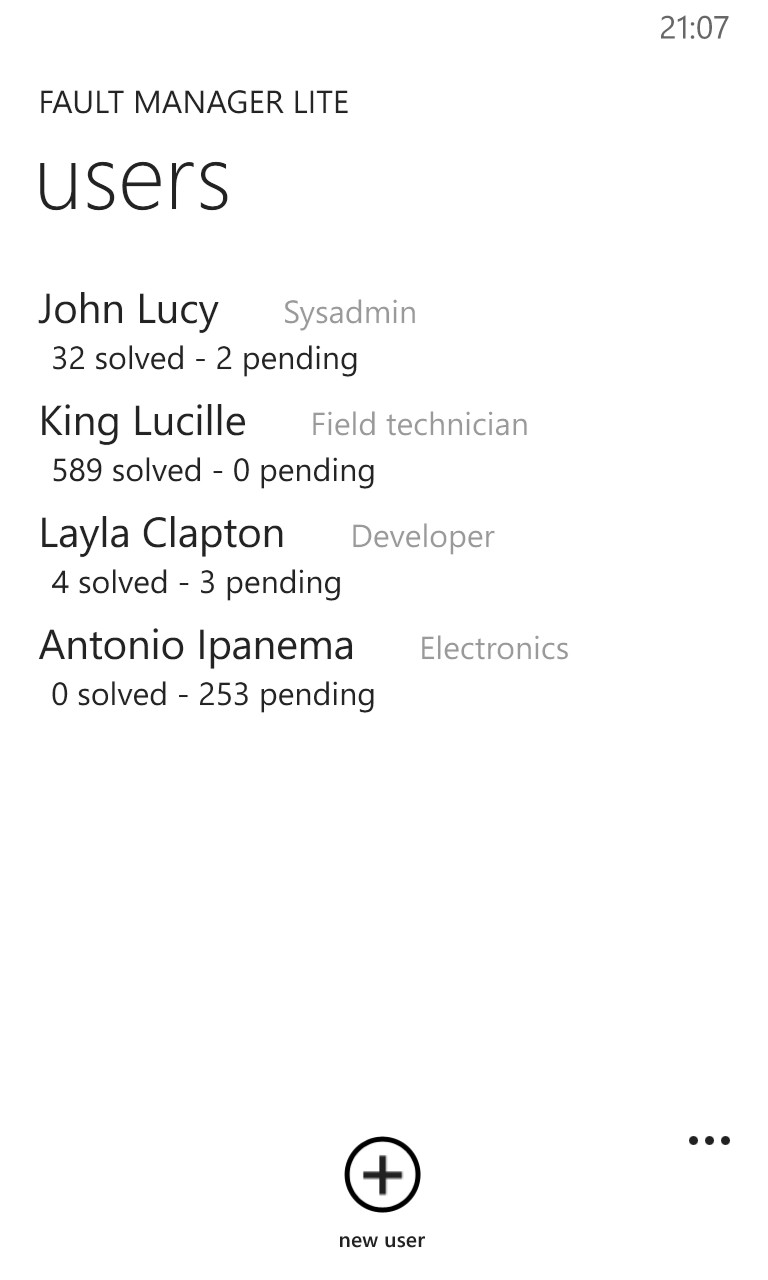
\includegraphics[width=\textwidth]{img/Users.jpg}
\end{minipage}
\caption{The managers will be able to see all the users, change their role or remove them.}
\label{imgUsers}
\end{figure}


As stated in the previous section, most of the code will be shared. This means that admins will mostly see the same screens as technicians with some minor tweaks. For example, when they list all the faults (figure \ref{imgFaultLog}), they will be able to assign them to any technician under their management.

The screens that are specific to admins are shown in figure \ref{imgUsers}, they're related to the user management subsystem.

\chapter{Conclusions}
\label{chapConclusions}

As we stated in the introduction, we think Triforce's solution, presented in this report, is the better tailored to solve current UAM's maintenance structure problems. We can deliver in a timely fashion a reliable, easy to use and useful system that can replace without hassle the currently deployed one.

Our proposal will allow us to listen to every user of the application and react accordingly, applying agile development techniques and continuous feedback and testing.

Fault Manager Lite will be easily and quickly deployed: because of our care and dedication to a polished user experience, formation will not be required for any user as the application and the system will be easy to use for everyone.

We consider the quality to price ratio of our proposal is high, and awarding the project to Triforce would be the best way to invest university assets  currently being wasted in an inefficient system.

\appendix

\chapter{Brainstorming}
\label{chapBrainstorming}

% -*- root: ../Technical_report.tex -*-
\section{Ideas about new development}

\subsection{Roles of the Application}

We define the user as the reporter of the incidence and the maintenance personnel as the people in charge of fixing the faults.

Every one uses the same application, but it will be shown a different menu depending on the role after the authentication.

\begin{itemize}
\item \textbf{Admin role: } The person or people in charge of banning and modifying manually what was automatically set by the system.

\item\textbf{Maintenance person:} You can see as a Maintenance person what task has been assigned to you and you can mark them as finished or as a false fault.

You can also ask for more information about the fault if it's not precise enough.

\item \textbf{User role: }  We may define subroles such as professor, student or workers (waiters, secretaries ... ) because of the liability of each group of people.

\end{itemize}

Everyone is a user and everyone can report faults but not  every one can be Maintenance person or user.

\subsection{Task priority}
We talked about 2 options:

\begin{itemize}
\item The user sets the priority of the task and the system has to take on account the liability of the user to set a real priority to the task.

\item There are tags and categories the user can add to the report and the system computes a real priority to the task.

Within this idea we need to add \textit{others} category, just in case.
\end{itemize}

\subsection{Location}

We have to distinguish 2 cases, if you are inside a building or not.

If you are not inside a building, the location will be automatic by GPS technology, but when faults are relative to inside of buildings material it will be necessary to ask the user the exact location. This will be ask by an interactive map.


We will also use WiFi location because sometimes GPS is a slow technology to be set and reliable.

\subsection{Manage task assignation}
The system automatically assigns tasks, depending on the location of the faults and the Maintenance person and the availability of the maintenance personnel.

Admin can set manually the task assignation.

We should take care of the following situation:

A Maintenance person works a lot and fix every task he was assigned, and, because he is free, the system assigns some more. On the other side, a Maintenance person is not working. As he has lot of pending task, system will not add more task to him. 

Plus, we can't just count the number of faults fixed, because there are ones more difficult than others. May be we should add \textit{difficulty of fault} depending on category to try control the how much job you have been assigned.

\subsection{Graphical interface}
We have Guille's application in which we will add just a profile page in which users can see
\begin{itemize}
\item the false faults they have reported .
\item the fault's reported state.
\end{itemize}

Every user's profile will be visible to the admin but he won't be able to see any personal data.

The admin can see profiles so before he can ban an user, he can check how many false and repeated faults he has reported.


\paragraph{Maintenance person interface}
The interface will show by color code the faults assignments classifying  they by pending, solved or not started.


\subsection{Repeated faults}
When an user is going to report a fault, the system will suggest if it's repeated showing possible faults. If the users says it's a new fault, it will be still marked as a possible repeated fault.

When a task is assigned to a Maintenance person, all possible repeated faults will be assigned to the same Maintenance person. It's Maintenance person's responsibility to say if they are the same or not.

If they are not the same, the task will be enqueued and the system will automatically be assigned to a Maintenance person, maybe the himself or may be not.


\subsection{Communication}

When a fault is fix, the system will notify the user who reported it.

\section{Questions to ask}

\begin{itemize}
\item When an emergency occurs in UAM (e.g., a fire, a flood...), does everyone get an alert?
\item Gamified experience? Do we ``reward'' the user for reporting faults or shall we instead offer detailed reports so the IT department can reward users as they want? (Credit's ETCS reward is possible, in the same way as languages)
\item We should take care of the following situation:

A Maintenance person works a lot and fix every task he was assigned, and, because he is free, the system assigns some more. On the other side, a Maintenance person is not working. As he has lot of pending task, system will not add more task to him. 

If he can assure us every one will work normally, that will solve the problem.
\end{itemize}




\chapter{Evaluate current technology}
\label{chapCurrentTechnology}

% -*- root: ../Technical_report.tex -*-
\section{Suggested webpages to look at}

Ivan's fault if this is empty xD

\section{Our own webpages to look at}

\subsection{Wunderlist}

\begin{itemize}
\item Nice interface to take into account for the task management.
\item Maybe shared list's so every handyman in science building can see pending task of others. (to ask)
\item See completed faults you fix. (pretty obvious).
\item Dead line for each fault, automatically set by the system taking into account the priority and the category. (to ask)
\end{itemize}


\subsection{Apple watch/YoApp/TapToTalk}

\begin{itemize}
\item Add some sort of really fast communication between handymen, so they don't have to call one another.
\item Add few types of default messages like “I'm going” or “Impossible” or “Need help”
\item Things to think about:
\begin{itemize}\label{AppleWatch}
\item ¿broadcast messages to all handyman? ¿Just to a few? Maybe making groups and you send notification to a group.
\item May be we should add some not so fast but more efficient communication way for handyman.
\end{itemize}
\end{itemize}

\subsection{Trello}

\begin{itemize}
\item Public taskboard that anyone can see? Only registered members?
\item Add one more state to task (pending, working, finished or impossible) better than wunderlist system (done or todo).
\end{itemize}

\subsection{Asana}
\begin{itemize}
 	\item  Dead line = due date or hour date??
\end{itemize}

\chapter{Meetings}
\label{chapMeetings}

% -*- root: ../Technical_report.tex -*-
\section{Meeting Announcements}
\subsection{Meeting Announcement - 1}

\textbf{From: } Iván Márquez Pardo

\textbf{To: } Guillermo Julián Moreno, Iván Márquez Pardo y Víctor de Juan Sanz.

\textbf{Date, Time and Place: } 27/01/2015 from 14:35 ultil we finish Brainstorming session in Science building, module 17.

\textbf{Purpose} Finish brainstorming session.

\subsection{Meeting Announcement - 2}


\textbf{From: }

\textbf{To: } Guillermo Julián Moreno, Iván Márquez Pardo y Víctor de Juan Sanz.


\textbf{Date, Time and Place: }


\textbf{Purpose: }


\textbf{Agenda: }

\textbf{Decision Follow-up: }


\textbf{Documentation: }


\section{Meetings Minutes}

We have excluded all in-class meetings. Should we add them?

\subsection{Meeting Minute - 1}


\textbf{Date and Time:} 27/01/2015 from 14:35 to 15:03.


\textbf{Participants: } Iván Márquez Pardo, Guillermo Julián Moreno y Víctor de Juan Sanz.


\textbf{Topics: }
Finish brainstorming and brainwriting session.


\textbf{Decitions Made: \\}

\begin{tabular}{|c|c|c|}
\hline Activity & Person Responsible & DeadLine \\\hline
Write down clearly all the ideas got from the brainstorming session & Víctor de Juan & 29/01/2015\\\hline

\end{tabular}

Brainstorm is finished, we have enough ideas to go to the next step.

\subsection{Meeting Minute - 2}


\textbf{Date and Time:}


\textbf{Participants: }

Iván Márquez Pardo, Guillermo Julián Moreno y Víctor de Juan Sanz.


\textbf{Topics: }

\textbf{Decitions Made: \\}

\begin{tabular}{|c|c|c|}
\hline Activity & Person Responsible & DeadLine \\\hline
olakase & olakase & olakase \\\hline

\end{tabular}

\chapter{Interview}
\label{chapInterview}
% -*- root: ../Technical_report.tex -*-

\newcommand{\interviewer}[1]{\vspace{12pt}\indent \textbf{#1}:\hspace{10pt} \itshape}
\newcommand{\interviewee}[1]{\\ \indent \upshape \textbf{#1}:\hspace{10pt}}

\newcommand{\tsc}{\interviewer{Triforce}}
\newcommand{\rsc}{\interviewee{Mr. Roberto}}
\newcommand{\ts}{\interviewer{T.}}
\newcommand{\rs}{\interviewee{R.}}

On February 10th 2015, we had an interview with the manager of the maintenance service of the UAM, Mr. Roberto. In the interview we clarified several aspects of the maintenance service in order to have a more detailed view of the problem and know by first hand how things are performed right now.

This section gathers the most important points of this interview between us, the Triforce representatives, and the maintenance manager.

\tsc Can you please tell us more about how is the maintenance service organized right now?
\rsc The maintenance service is quite decentralized in several groups depending on the tasks they perform. These groups are auto-organized, assigning repair tasks on their own and they don't contact me usually. This division into independent groups and the lack of coordination between them sometimes cause some budget and personnel problems.

\tsc So, basically, you want us to try to centralize the maintenance service to sistematize the task assignment, right?
\rsc Yes, indeed.

\ts How many different departments are there in total?
\rs There are 9 different departments: Information Technologies, Electricity, Plumbers, Elevators, Heating, Air conditioning, Cleaning, Gardeners and Garbage collectors.

\ts And you said they are auto-organized, but how?
\rs They all received their corresponding repair tasks and they are manually assigned to members of each department. However, there are two departments that work in a different way: the Cleaning and the Information Technologies department.

\ts Can you give us more details about the Cleaning department?
\rs Yes. The Cleaning department is formed by 8 different cleaning companies, each of those has a manager for the building they are in charge of. Your application should take that into account, because cleaning tasks will be assigned to the cleaning manager of the building the fault has been encountered. As they are different companies, that manager will internally assign that task to one of its employees; your application should not interfere in that.

\ts And what about the Information Technologies department? How do they organise?
\rs Well, the Information Technologies department has its own application to automatically assign tasks. Their application is based on emails which are sent by the users, who fill a form in the maintenance service website. The system reads those emails and assigns the repair task automatically to a member of the technical staff; if it can't assign it automatically, then the manager of this department reads it and assigns it manually.

\ts You want us to overwrite this system or maintain it along with our app?
\rs The organization of the Information Technologies department should be the same as the others, so this system must disappear when you finish setting up your app.

\ts Ok, we will overwrite the IT system... Can we count on their collaboration?
\rs Yes, the whole maintenance service has agreed to start using your app in order to encourage the collaboration and coordination between departments.

\ts Perfect. We have clarified some details of the old organization of the maintenance service, now let's concentrate on the new organization, our application. Are the staff used to mobile phones?
\rs Yes, they are used to smartphones, but the more user-friendly you could make your app, the better.

\ts We will take it into account while making the mock-ups, don't worry about it. We had thought that it could be useful to include a system of alerts and notifications so that, in case of emergency (fire in a building, for example), a user could press a big button and all the other users of the app would receive an alert telling them information about the danger and its location.
\rs It could be useful, indeed. It is a good idea to include it in the app.

\ts We are pleased you like it. Would you like us to also include statistics of faults so that the manager could visualize them?
\rs For me, it is pointless to create any type of statistics about faults. The only thing I need is a fault history, but no fault statistics.

\ts In that case, fault statistics discarded. We thought that the urgency of faults should be set automatically, but users could classify faults as urgent while filling the report and their opinion would be automatically taken into account depending on their previous reports. Is this correct for you?
\rs In the beginning, yes, it is. But there is one thing I need you to include: I must be able to classify manually a fault as urgent in order to be able to accelerate certain repairs.

\ts No problem, we will include that option in our system. One last question: what happens if users are not able to identify the category of a fault, how can we assign it to the corresponding member of the technical staff? For example, if there is a problem with the watering system and the user does not know if its a problem of plumbery or for the gardeners, what do we do with that report?
\rs In case there are any unclassified or extraordinary reports, I, as general maintenance manager, will be in charge of reading them and manually assign their repair task to the correct technician.

\ts Perfect, in that case, we have finished our interview. Thank you for your help, Mr. Roberto.
\rs You are welcome, I am looking forward to see your application.



\end{document}
